\documentclass[11pt]{standalone}

\usepackage{helvet}

\usepackage{ifthen}
\usepackage{tikz} 
\usetikzlibrary{shapes.misc}
\usetikzlibrary{arrows,arrows.meta}
\usetikzlibrary{calc,intersections, patterns, math}
\usetikzlibrary{patterns, animations}
\usetikzlibrary{decorations}
\usetikzlibrary{decorations.text}
\usetikzlibrary{decorations.pathmorphing}

\definecolor{pfeil}{RGB}{168,167,167}
\definecolor{petrol}{RGB}{0, 118, 136}
\definecolor{darkgoldenrod}{RGB}{184, 134, 11}
\colorlet{petrol-lighter}{petrol!40}
\colorlet{darkgoldenrod-lighter}{darkgoldenrod!40}

\begin{document}

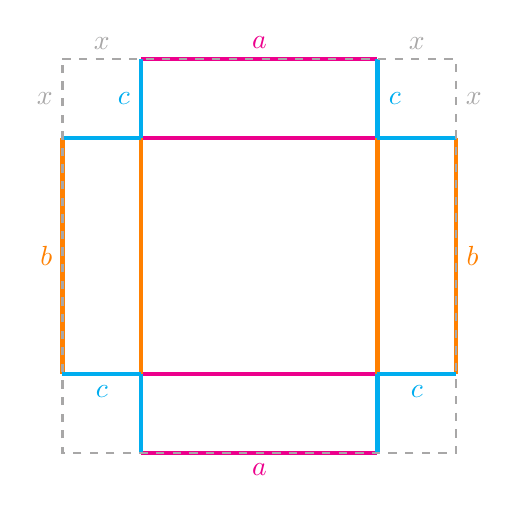
\begin{tikzpicture}[pfeil]

    % \draw[thick, fill=petrol!20, draw=petrol-lighter, rounded corners=2ex, opacity=0.5] (0,0) rectangle ++ (1.5,3.5);
    % \draw[thick, fill=darkgoldenrod!20, draw=darkgoldenrod-lighter, rounded corners=2ex, opacity=0.5] (5,0) rectangle ++ (1.5,3.5);

    \draw[ultra thick, magenta] (1,0) -- (4,0);
    \draw[ultra thick, magenta] (1,-1) -- (4,-1);
    \draw[ultra thick, magenta] (1,-4) -- (4,-4);
    \draw[ultra thick, magenta] (1,-5) -- (4,-5);

    \draw[ultra thick, orange] (0,-1) -- (0,-4);
    \draw[ultra thick, orange] (1,-1) -- (1,-4);
    \draw[ultra thick, orange] (4,-1) -- (4,-4);
    \draw[ultra thick, orange] (5,-1) -- (5,-4);

    \draw[ultra thick, cyan] (1,0) -- node[left] {\color{cyan}$c$} (1,-1);
    \draw[ultra thick, cyan] (1,-4) -- (1,-5);
    \draw[ultra thick, cyan] (4,0) -- node[right] {\color{cyan}$c$} (4,-1);
    \draw[ultra thick, cyan] (4,-4) -- (4,-5);

    \draw[ultra thick, cyan] (0,-1) -- (1,-1);
    \draw[ultra thick, cyan] (0,-4) -- node[below] {\color{cyan}$c$} (1,-4);
    \draw[ultra thick, cyan] (4,-1) -- (5,-1);
    \draw[ultra thick, cyan] (4,-4) -- node[below] {\color{cyan}$c$} (5,-4);

    \path (0,0) -- node[above] {$x$} (1,0);
    \path (0,0) -- node[left] {$x$} (0,-1);
    \path (4,0) -- node[above] {$x$} (5,0);
    \path (5,0) -- node[right] {$x$} (5,-1);

    \draw[thick, dashed] (0,0) -- node[above] {\color{magenta}$a$} (5,0) -- node[right] {\color{orange}$b$} (5,-5) 
                -- node[below] {\color{magenta}$a$} (0,-5) -- node[left] {\color{orange}$b$} cycle;
    

    


\end{tikzpicture}

\end{document}
